\chapter{Grundlagen}

Um zu verstehen, wie Transformer funktionieren, muss zunächst ein kurzer Überblick über neuronale Netze gegeben werden.  

\section{Neuronale Netze}

Neuronale Netze sind ein Teilgebiet des maschinellen Lernens.
Sie sind trainierbar und können die gesammelten Erfahrungen auf neue Daten anwenden.  
Neuronale Netze orientieren sich an der Struktur des menschlichen Gehirns (vgl. \cite[S. 14]{Kinnebrock.2018}).  
Sie bestehen aus mehreren Schichten von Neuronen (vgl. \cite[S. 25]{Kinnebrock.2018}).  

Es gibt dabei eine Eingabe- und Ausgabeschicht sowie mehrere versteckte Schichten, in denen die eigentliche Verarbeitung stattfindet.  
Jedes Neuron verarbeitet seine eigenen Daten, gewichtet sie und addiert sie mit den Ergebnissen der vorherigen Schicht.  
Dieses Ergebnis wird dann an die Aktivierungsfunktion weitergegeben, um die nächsten verbundenen Neuronen anzusteuern.  
Diese Funktion bestimmt, ob das Neuron \enquote{feuert} und das Signal weitergeleitet wird (vgl. \cite[S. 14]{Kinnebrock.2018}).  

Über die Jahre haben sich neuronale Netze besonders für Anwendungen wie Bildanalysen als äußerst effektiv erwiesen (vgl. \cite[S. 16]{paass.2020}).  
Doch ein Problem war lange die Textanalyse und -verarbeitung (vgl. \cite[S. 22]{paass.2020}).
Hier besteht die Herausforderung darin, dass Informationen nicht wie bei einem Bild simultan erfasst werden können.  
Um den Sinn eines Satzes zu verstehen, muss der Inhalt schrittweise verarbeitet werden.  

\section{Neuronale Netze für Textverarbeitung}

Für Textanalysen, Übersetzungen oder Zusammenfassungen wurden lange Zeit Recurrent Neural Networks (RNNs) verwendet (siehe Abb. \fig{ref:rnn}).  
RNNs analysieren einen Text sequentiell und verknüpfen jedes Wort mit dem Kontext aus dem vorhergehenden Wort (vgl. \cite[S. 2]{attention}).


\begin{figure}[ht]
	\centering
	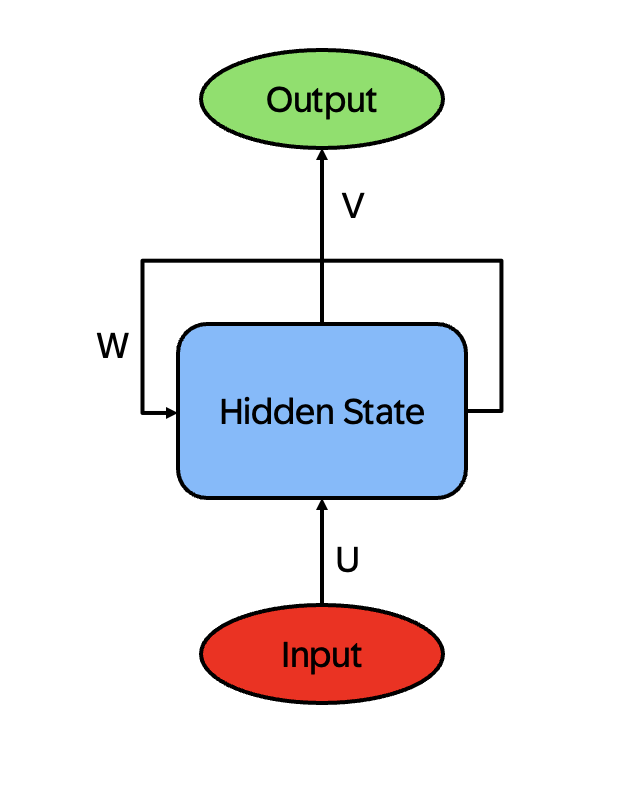
\includegraphics[width=0.3\textwidth]{Bilder/RNN.png}
	\caption{RNN als Vorgänger zum Transformer}
	\label{fig:rnn}
\end{figure}

Doch RNNs haben Schwächen (vgl. \cite[S. 2]{attention}) (vgl. \cite[S. 208]{paass.2020}).
Sie haben Schwierigkeiten, den Kontext von größeren Texten vollständig zu erfassen.  
Außerdem ist die sequentielle Verarbeitung ineffizient und schlecht auf moderne Hardware optimiert, die auf Parallelverarbeitung ausgelegt ist.  

Um diese Probleme zu lösen, wurde eine neue Art neuronaler Netze entwickelt: die Transformer.
